\documentclass{standalone}

\usepackage{tikz}
\usepackage{circuitikz}

\tikzset{block/.style = {draw, fill=white, very thick, rectangle, minimum height=1cm, minimum width=2cm},
         lblock/.style={draw,fill=white,very thick, rectangle, minimum height=3cm, minimum width=1cm},
         sum/.style= {draw, fill=white, very thick, circle, node distance=0.5cm}}

         
\begin{document}
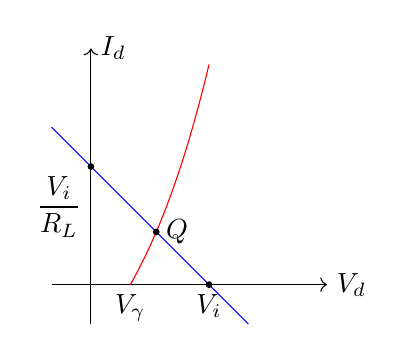
\begin{tikzpicture}[scale=2]
    \draw[->](-0.25,0)--(1.5,0)node[right]{$V_d$};
    \draw[->](0,-0.25)--(0,1.5)node[right]{$I_d$};

    \node[below] at(0.25,0){$V_{\gamma}$};
    \draw[red,smooth, domain=0.25:0.75]plot (\x, {e^(1.75*(\x-0.25))-1});

    \draw[blue](-0.25,1)--(1,-0.25);
    \filldraw[black](0.415,0.335)circle(0.5pt);
    \node[right]at(0.415,0.335){$Q$};
    \filldraw[black](0,0.75)circle(0.5pt);
    \filldraw[black](0.75,0)circle(0.5pt);
    \node[below left]at(0,0.75){$\displaystyle\frac{V_i}{R_L}$};
    \node[below]at(0.75,0){$V_i$};
\end{tikzpicture}
\end{document}